\documentclass[12pt,a4paper]{article}
\usepackage{fontspec}
\defaultfontfeatures{Mapping=tex-text}
\usepackage{xunicode}
\usepackage{xltxtra}
%\setmainfont{???}
\usepackage{amsmath}
\usepackage{amsfonts}
\usepackage{amssymb}
\usepackage{tabularx}
\usepackage{float}
\usepackage{hyperref}
\usepackage{listings}
\usepackage[a4paper, inner=2.5cm, outer=2.5cm, top=2cm, bottom=3cm]{geometry}
\usepackage{parskip}


\usepackage{subcaption}

\usepackage{graphicx}
\graphicspath{{./images/Task1/} {./images/Task2/} {./images/Task3/} {./images/Task2_1/} {./images/Task2_2/} {./images/Task2_3/}}


\author{Richard Amering - Francisco Goio}



\newcommand\musteq{\stackrel{\normalfont\mbox{!}}{ = }}
\newcommand{\etal}{\textit{et al}. }
\newcommand{\ie}{\textit{i}.\textit{e}. }
\newcommand{\eg}{\textit{e}.\textit{g}.\ }

\newtoks\rowvectoks
\newcommand{\rowvec}[2]{%
  \rowvectoks={#2}\count255=#1\relax
  \advance\count255 by -1
  \rowvecnexta}
\newcommand{\rowvecnexta}{%
  \ifnum\count255>0
    \expandafter\rowvecnextb
  \else
    \begin{pmatrix}\the\rowvectoks\end{pmatrix}
  \fi}
\newcommand\rowvecnextb[1]{%
    \rowvectoks=\expandafter{\the\rowvectoks&#1}%
    \advance\count255 by -1
    \rowvecnexta}
    
    

\begin{document}

\begin{titlepage}
%%%%%%%%% begin snippet
%% You need to add the package "tabularx".
%% Place the snippet right after \begin{document}

% need tabularx
% \usepackage{tabularx}

\begin{titlepage}
              \begin{center}
             \begin{huge}
				   %% Update assignment number here
                   \textbf{Assignment 1}
             \end{huge}
       \end{center}

       \begin{center}
             \begin{large}
                   Deep Learning 1, SS22
             \end{large}
       \end{center}

       \begin{center}
 \begin{tabularx}{\textwidth}{|>{\hsize=.33\hsize}X|>{\hsize=.33\hsize}X|>{\hsize=.33\hsize}X|} 

                   \hline
                   \multicolumn{3}{|c|}{\textbf{Team Members}} \\
                   \hline
                   Last name & First name & Matriculation Number \\
                   \hline
                   Amering & Richard & 1331945 \\
                   \hline

             \end{tabularx}
       \end{center}

\end{titlepage}


%%%%%%%%% end snippet

\end{titlepage}




\newpage 

\section{Problem description: Neural Networks: Regression}
The objective of this assignment is to design a regression problem using the provided dataset on social capital. The dataset was downloaded from the following website:

https://data.humdata.org/dataset/social-capital-atlas

This regression problem will be modeled with a neural network using the Python tools Tensorflow 2.0 and Keras. Different settings (architecture, optimizer, activation, ...) of the neural network will be explored to get the best fit for the chosen dataset.

\subsection*{1.1 Preprocessing of the raw data}

The first task of the practical is to choose a dataset, and from that create separate training and test datasets randomly. The training set should contain 80 \% of the data and the test data 20 \%. The chosen dataset is ’social\_capital\_zip.csv’. We decided to normalize the data, as suggested in the assignment, to values between zero and one with the following equation:
\[x_{i,normalized} = \frac{x_{i}-x_{min}}{x_{max}-x_{min}}\]

\subsection*{1.2 Definition of the regression problem}
For design the regression problem input and output variables must be chosen. As input this set of variables was chosen: 
'ec\_zip', 'ec\_se\_zip', 'nbhd\_ec\_zip', 'ec\_grp\_mem\_zip', 'ec\_high\_zip', 'ec\_high\_se\_zip', 'nbhd\_ec\_high\_zip', 'ec\_grp\_mem\_high\_zip', 'exposure\_grp\_mem\_zip', 'exposure\_grp\_mem\_high\_zip', 'nbhd\_exposure\_zip', 'bias\_grp\_mem\_zip', 'bias\_grp\_mem\_high\_zip', 'nbhd\_bias\_zip', 'nbhd\_bias\_high\_zip', 'clustering\_zip', 'support\_ratio\_zip'. 
The reason for this is that with a larger amount of information, the neural network is better able to detect statistical patterns for which it is not trivial to understand whether they affect the output parameters. Only the "zip", "county", "num\_below\_p50" and "pop2018" data were not included because we assume that these data (e.g., the number of counties) do not affect the social metrics.
The two output variables which are:
\begin{itemize}
  \item volunteering rate zip
  \\This variable describes the percentage of Facebook users who are members of a group that is assumed to be about ‘volunteering’ or ‘activism’ based on the group title and other group characteristics.
  \item civic organizations zip
  \\The second variable describes the number of Facebook pages predicted to be "common good" pages based on page title, category, and other page characteristics, per 1,000 users in the zip code.
\end{itemize}

\subsection*{1.3 Architecture and activation of the neural network}
As validation set for our neural network 20 \% out of the training data randomly was chosen. With this data the network was validated. For all our evaluations the batch size was set to 64 and 50 epochs were trained. We decided to investigate three different neural network structures and two different activation functions. The structures are: \newline$[17, 32, 8, 32, 2]$, $[17, 32, 32, 2]$, $[17, 8, 8, 2]$\newline The first character is the number of input neurons, which is fixed for all inputs, since we have the same amount of input data for all variants. The same is true for the last character, which is the output layer and always contains two neurons. The numbers between these two indicate how many neurons each hidden layer has. For the activation function the ReLU and the sigmoid function were investigated. 

\subsection*{1.4 Optimizers and learning rates of the neural network}
As for the learning rate also an exponential decay function was used to adjust the learning rate while training.
Values for Exponential Decay are: 
$initial\ learing\ rate =  10^-3$, 
$decay\ steps=20$, 
$decay\ rate=0.9$
All in all three different optimizers were invenstigated: ADAM, SGD and SGD Momentum. The momentum for the SGD Momentum was:
$SGD\ Momentum= 0.5$
Table \ref{table:overview_table} shows all the investigated combinations of optimizers, network structures, activation function and learning rates, along with the respective loss on the validation set. The table is ordered from lowest loss (best model) to highest loss (worst model). It appears that the Adam optimizer generaly performs best, since all hyperparameter combinations with this optimizer are among the best performers, and no architecture with it appears in the lower half of the ranking. SGD and SGD-momentum perform about equally, with some good results and some bad results. We could not conclude that one architecture is generaly superior to the others.
We conclude that the Adam optimizer with a network structure of [17, 32, 8, 32, 2] neurons, ReLU activation function and a constant learning rate of 0.0001 would perform best.
We therefore set up a new model with the optimal parameters, recombine our training- and validation set, and evaluate our new optimal model against the test set, which is so far not being used.
\begin{table}[H]
    \centering
    \begin{tabular}{|c|c|c|c|c|}
    \hline
        Optimizer & Structure & Activation function & Learning Rate & Validation Loss \\ \hline
        Adam & [17, 32, 8, 32, 2] & relu & 0.0001 & 0.00143 \\ \hline
        Adam & [17, 32, 32, 2] & relu & 0.0001 & 0.00153 \\ \hline
        Adam & [17, 8, 8, 2] & relu & 0.0001 & 0.00155 \\ \hline
        Adam & [17, 32, 32, 2] & sigmoid & 0.0001 & 0.00156 \\ \hline
        Adam & [17, 32, 8, 32, 2] & relu & Exp. dec. & 0.00161 \\ \hline
        Adam & [17, 8, 8, 2] & sigmoid & 0.0001 & 0.00165 \\ \hline
        Adam & [17, 32, 8, 32, 2] & sigmoid & 0.0001 & 0.00169 \\ \hline
        Adam & [17, 8, 8, 2] & relu & Exp. dec. & 0.00169 \\ \hline
        SGD-Mom & [17, 8, 8, 2] & sigmoid & 0.0001 & 0.00186 \\ \hline
        Adam & [17, 32, 32, 2] & relu & Exp. dec. & 0.00190 \\ \hline
        Adam & [17, 32, 8, 32, 2] & sigmoid & Exp. dec. & 0.00190 \\ \hline
        SGD-Mom & [17, 32, 8, 32, 2] & sigmoid & 0.0001 & 0.00192 \\ \hline
        Adam & [17, 32, 32, 2] & sigmoid & Exp. dec. & 0.00193 \\ \hline
        SGD-Mom & [17, 32, 32, 2] & sigmoid & Exp. dec. & 0.00201 \\ \hline
        SGD & [17, 32, 8, 32, 2] & sigmoid & 0.0001 & 0.00213 \\ \hline
        SGD & [17, 32, 32, 2] & sigmoid & 0.0001 & 0.00217 \\ \hline
        SGD-Mom & [17, 32, 32, 2] & sigmoid & 0.0001 & 0.00224 \\ \hline
        Adam & [17, 8, 8, 2] & sigmoid & Exp. dec. & 0.00238 \\ \hline
        SGD & [17, 32, 8, 32, 2] & relu & 0.0001 & 0.00255 \\ \hline
        SGD-Mom & [17, 32, 8, 32, 2] & relu & 0.0001 & 0.00258 \\ \hline
        SGD-Mom & [17, 8, 8, 2] & relu & 0.0001 & 0.00316 \\ \hline
        SGD & [17, 32, 32, 2] & relu & 0.0001 & 0.00353 \\ \hline
        SGD-Mom & [17, 32, 8, 32, 2] & sigmoid & Exp. dec. & 0.00362 \\ \hline
        SGD-Mom & [17, 32, 32, 2] & relu & Exp. dec. & 0.00378 \\ \hline
        SGD & [17, 8, 8, 2] & sigmoid & 0.0001 & 0.00385 \\ \hline
        SGD-Mom & [17, 32, 32, 2] & relu & 0.0001 & 0.00390 \\ \hline
        SGD & [17, 8, 8, 2] & relu & 0.0001 & 0.00436 \\ \hline
        SGD-Mom & [17, 32, 8, 32, 2] & relu & Exp. dec. & 0.00461 \\ \hline
        SGD & [17, 32, 8, 32, 2] & sigmoid & Exp. dec. & 0.00699 \\ \hline
        SGD-Mom & [17, 8, 8, 2] & relu & Exp. dec. & 0.00737 \\ \hline
        SGD & [17, 8, 8, 2] & relu & Exp. dec. & 0.00773 \\ \hline
        SGD & [17, 32, 8, 32, 2] & relu & Exp. dec. & 0.01240 \\ \hline
        SGD & [17, 32, 32, 2] & sigmoid & Exp. dec. & 0.01598 \\ \hline
        SGD & [17, 8, 8, 2] & sigmoid & Exp. dec. & 0.01620 \\ \hline
        SGD & [17, 32, 32, 2] & relu & Exp. dec. & 0.03388 \\ \hline
        SGD-Mom & [17, 8, 8, 2] & sigmoid & Exp. dec. & 0.04600 \\ \hline
    \end{tabular}  
    \caption{Overview of hyperparameter combinations with corresponding validation loss}
    \label{table:overview_table}
\end{table}

\subsection*{1.5 Final test evaluation of best setup}
Figure \ref{fig:best_model} shows the training performance for our best model based on previous validations. The best training loss achieved on the combined training set was 0.0016, while the final test-loss was 0.00192. This suggests that there is a slight bit of overfitting, which we find not to serious to require further counter meassures. If overfitting would become too strong, regularization techniques could be employed, for example L1 or L2 regularization.

\begin{figure}[H]
    \centering
    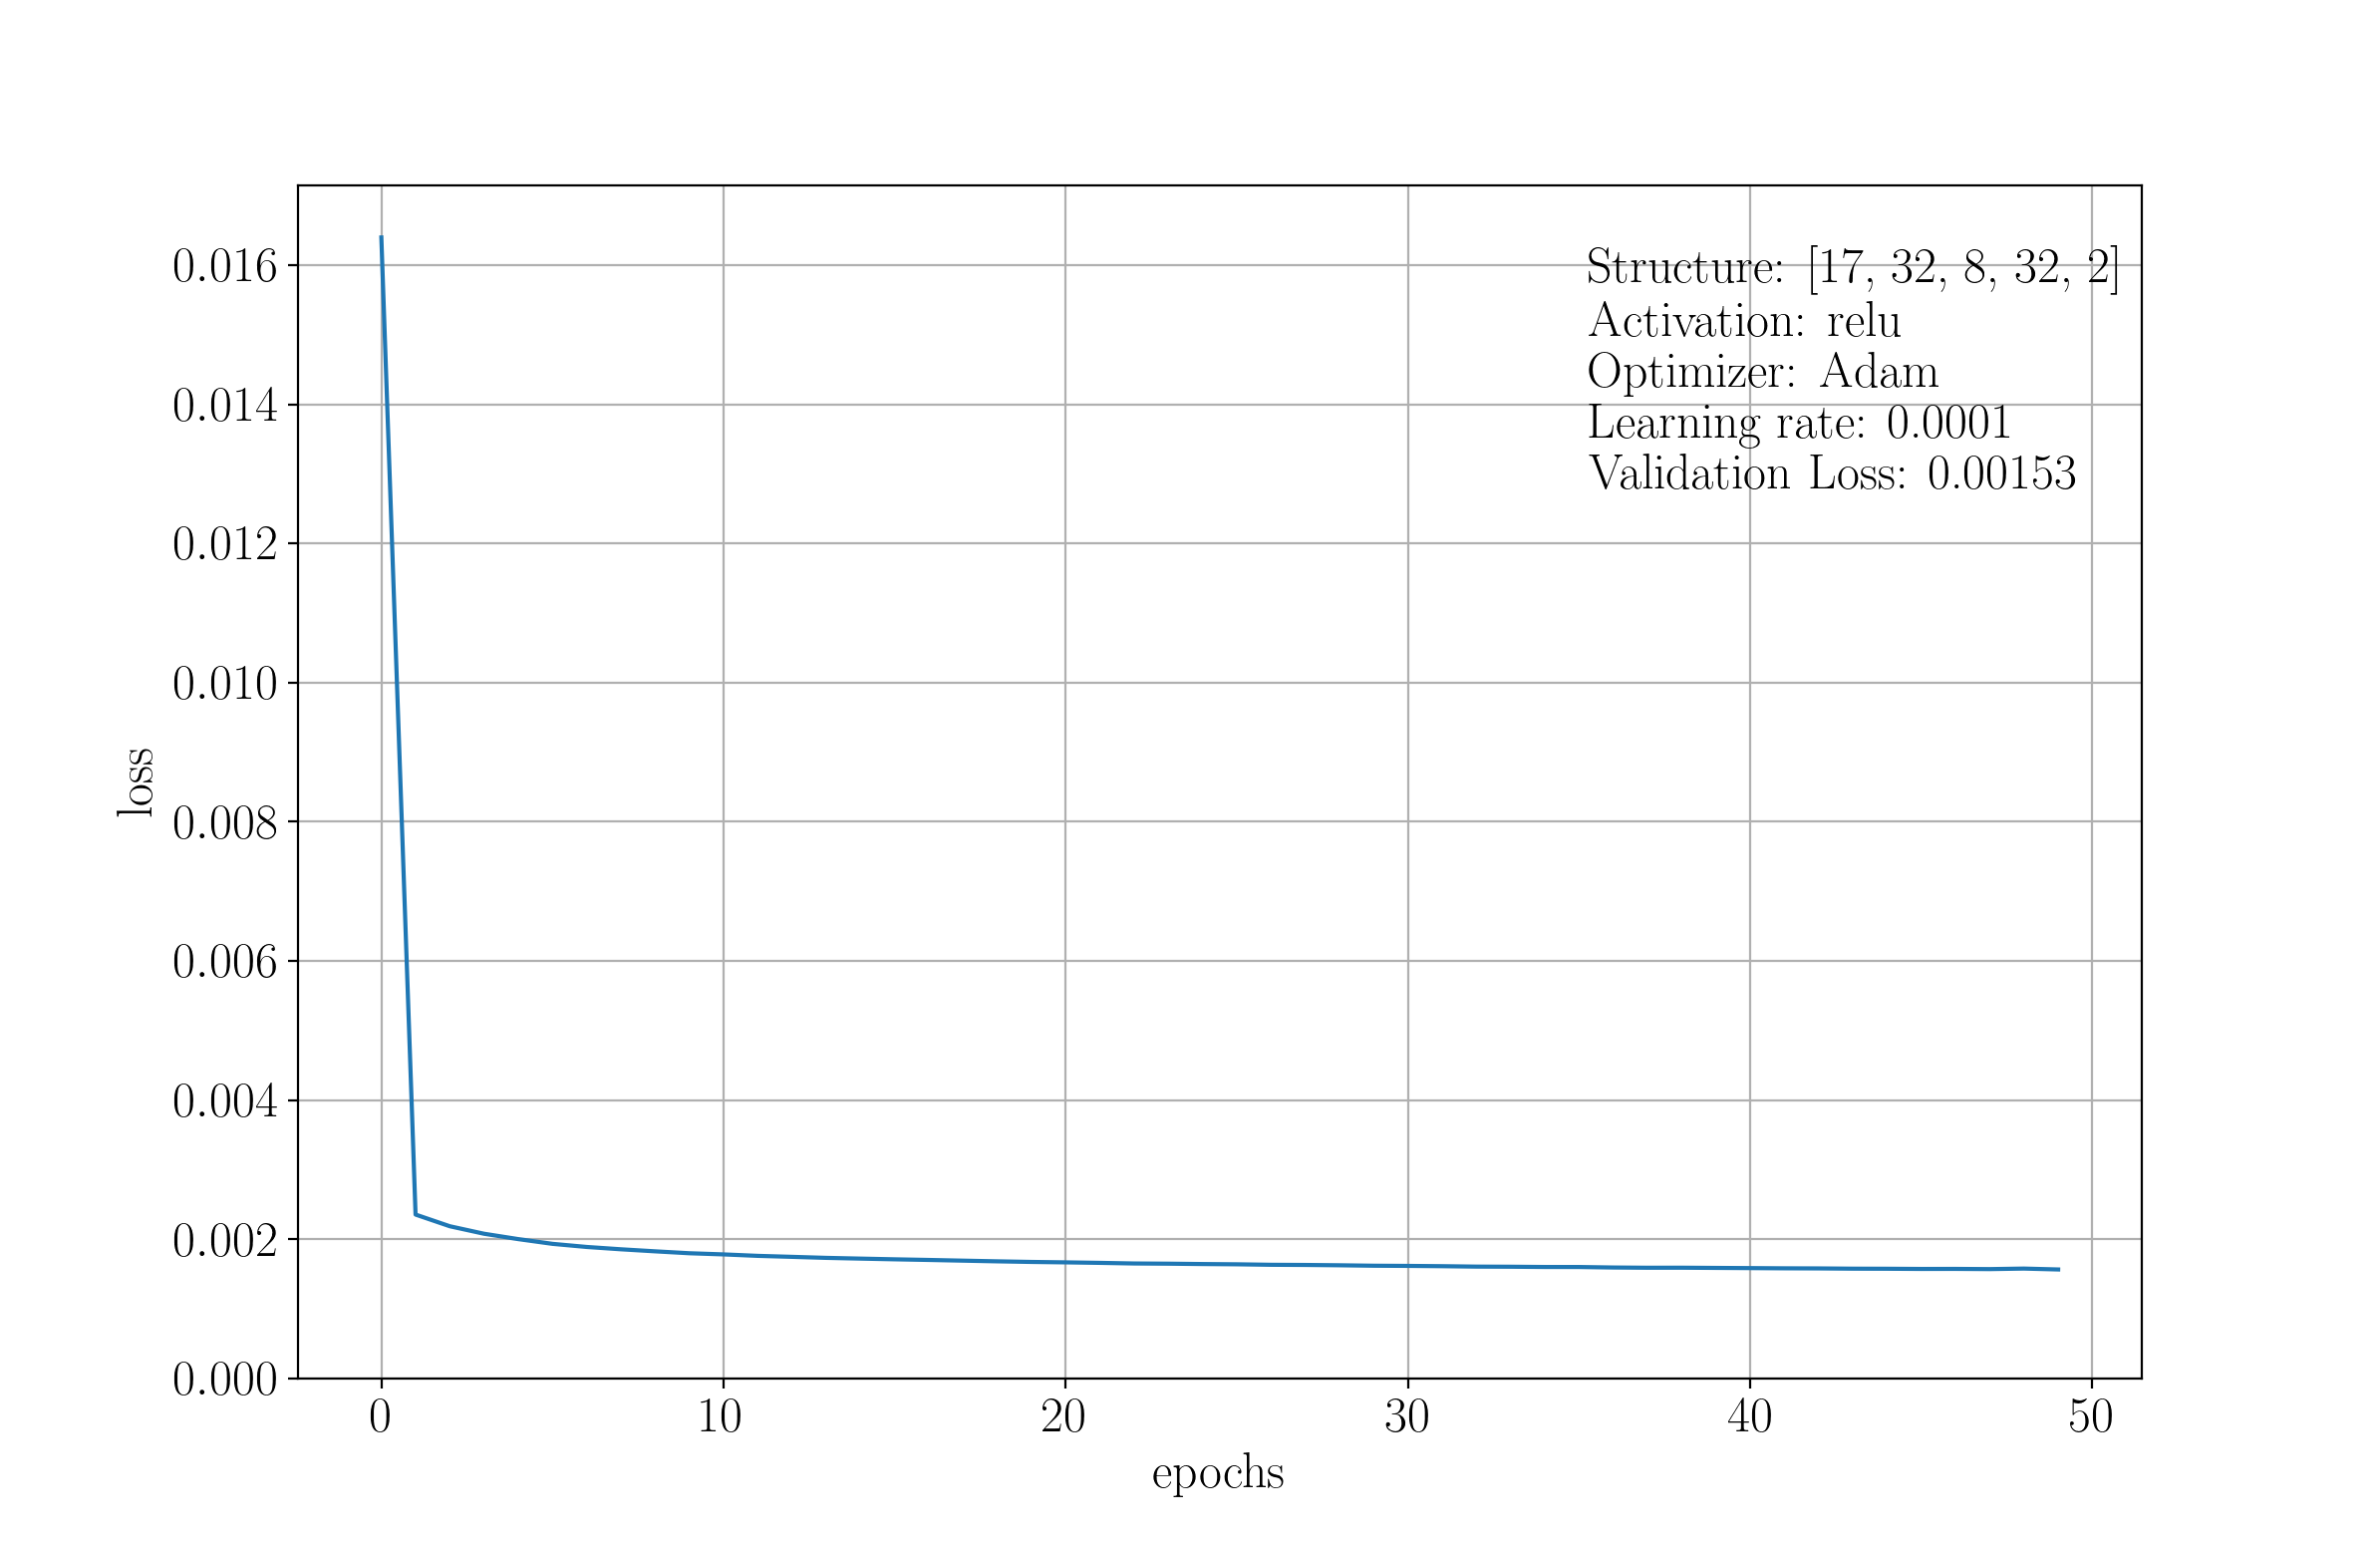
\includegraphics[width=1\linewidth]{training_evolution_best_model.png}  
    \caption{Training loss for the best performing model}
    \label{fig:best_model}
\end{figure}



\end{document}